% ============================================================
%  Chapter 8: Exponents, Radicals & Exponential Functions
%  Compile with: pdflatex exponents_textbook.tex  (twice)
% ============================================================
\documentclass[12pt, letterpaper]{book}

% ── Packages ────────────────────────────────────────────────
\usepackage[margin=1in, left=1.2in]{geometry}
\usepackage{amsmath, amssymb, amsthm}
\usepackage{mathtools}
\usepackage{array, booktabs, tabularx}
\usepackage{xcolor}
\usepackage{tcolorbox}
\usepackage{enumitem}
\usepackage{multicol}
\usepackage{tikz}
\usepackage{pgfplots}
\usepackage{fancyhdr}
\usepackage{titlesec}
\usepackage{parskip}
\usepackage{mdframed}
\usepackage{hyperref}
\usepackage{fontenc}
\usepackage{microtype}

\pgfplotsset{compat=1.18}
\tcbuselibrary{skins, breakable, theorems}

% ── Colors ──────────────────────────────────────────────────
\definecolor{AccentRed}{RGB}{139, 32, 32}
\definecolor{Gold}{RGB}{201, 150, 58}
\definecolor{PaperBg}{RGB}{250, 247, 242}
\definecolor{DefBg}{RGB}{253, 245, 230}
\definecolor{ExBg}{RGB}{245, 240, 255}
\definecolor{ExBorder}{RGB}{107, 70, 193}
\definecolor{NoteBg}{RGB}{255, 248, 225}
\definecolor{GreenOK}{RGB}{56, 161, 105}
\definecolor{LightRule}{RGB}{212, 201, 176}

% ── Page style ──────────────────────────────────────────────
\pagestyle{fancy}
\fancyhf{}
\fancyhead[LE]{\small\textit{Chapter 8 · Exponents, Radicals \& Exponential Functions}}
\fancyhead[RO]{\small\textit{\leftmark}}
\fancyfoot[C]{\small· \thepage ·}
\renewcommand{\headrulewidth}{0.4pt}

% ── Section title formatting ────────────────────────────────
\titleformat{\chapter}[display]
  {\normalfont\huge\bfseries\color{AccentRed}}
  {\small\scshape Chapter \thechapter}{10pt}{\Huge}
\titleformat{\section}
  {\normalfont\Large\bfseries\color{AccentRed}}
  {\thesection}{0.8em}{}[\titlerule]
\titleformat{\subsection}
  {\normalfont\large\bfseries\itshape\color{black!80}}
  {\thesubsection}{0.6em}{}

% ── tcolorbox environments ───────────────────────────────────

% Definition box (gold)
\tcbset{
  defstyle/.style={
    enhanced, breakable,
    colback=DefBg, colframe=Gold,
    leftrule=5pt, toprule=1pt, bottomrule=1pt, rightrule=1pt,
    arc=2pt, outer arc=2pt,
    fonttitle=\bfseries\color{Gold!80!black},
    attach boxed title to top left={yshift=-2mm, xshift=6mm},
    boxed title style={colback=Gold, colframe=Gold, arc=2pt},
  }
}

\newtcolorbox{definitionbox}[1][]{defstyle, title={Definition: #1}}

% Example box (purple)
\tcbset{
  exstyle/.style={
    enhanced, breakable,
    colback=ExBg, colframe=ExBorder,
    leftrule=5pt, toprule=1pt, bottomrule=1pt, rightrule=1pt,
    arc=2pt,
    fonttitle=\bfseries\color{ExBorder!80!black},
    attach boxed title to top left={yshift=-2mm, xshift=6mm},
    boxed title style={colback=ExBorder, colframe=ExBorder, arc=2pt},
  }
}

\newtcolorbox{examplebox}[1][]{exstyle, title={Worked Example: #1}}

% Story / narrative callout (gold border, light yellow)
\newtcolorbox{storybox}{
  enhanced, breakable,
  colback=NoteBg, colframe=Gold,
  arc=4pt, outer arc=4pt,
  leftrule=1.5pt, toprule=1.5pt, bottomrule=1.5pt, rightrule=1.5pt,
  left=8pt, right=8pt, top=8pt, bottom=8pt,
  before upper={\itshape},
}

% Answer key box (green)
\newtcolorbox{answerbox}[1][]{
  enhanced, breakable,
  colback=GreenOK!8, colframe=GreenOK,
  leftrule=4pt, arc=2pt,
  fonttitle=\bfseries\color{GreenOK!70!black},
  attach boxed title to top left={yshift=-2mm, xshift=6mm},
  boxed title style={colback=GreenOK, colframe=GreenOK, arc=2pt},
  title={#1}
}

% Law card (for the five laws grid)
\newtcolorbox{lawcard}[1]{
  enhanced,
  colback=white, colframe=LightRule,
  borderline north={3pt}{0pt}{AccentRed},
  arc=0pt, outer arc=0pt,
  title={\footnotesize\ttfamily\color{AccentRed}\MakeUppercase{#1}},
  fontupper=\itshape,
  left=6pt, right=6pt, top=6pt, bottom=6pt,
}

% ── Worksheet answer line ────────────────────────────────────
\newcommand{\ansline}{\underline{\hspace{6cm}}}
\newcommand{\shortansline}{\underline{\hspace{3.5cm}}}

% ── Misc helpers ─────────────────────────────────────────────
\newcommand{\nthroot}[2]{\sqrt[\leftroot{-1}\uproot{2}#1]{#2}}

% ============================================================
\newcommand{\circled}[1]{\raisebox{.5pt}{\textcircled{\raisebox{-.9pt}{#1}}}}
\begin{document}
% ============================================================

% ── Title page ──────────────────────────────────────────────
\begin{titlepage}
  \centering
  \vspace*{3cm}
  {\small\scshape\color{AccentRed} Chapter 8}\par
  \vspace{0.5cm}
  {\Huge\bfseries Exponents, Radicals\\[6pt] \& Exponential Functions}\par
  \vspace{0.4cm}
  {\large\color{Gold}\rule{6cm}{1.5pt}}\par
  \vspace{1.2cm}
  \begin{storybox}
    Imagine filling a chess board with grains of rice: one grain on the first square,
    two on the second, four on the third --- each square doubling the last.
    By square 64, you would need more rice than has ever been grown on Earth.
    This astonishing growth is the power of exponents. In this chapter we will
    build the rules that govern that power, learn how to undo it with radicals,
    and explore the beautiful curves that exponential functions trace across the plane.
  \end{storybox}
  \vspace{1.2cm}
  \begin{flushleft}
    \large
    \textbf{Section 8.1} \quad The Laws (Properties) of Exponents\\[4pt]
    \textbf{Section 8.2} \quad Radical Notation \& Rational Exponents\\[4pt]
    \textbf{Section 8.3} \quad The Exponential Function $y = 2^x$
  \end{flushleft}
  \vfill
  {\small\color{gray} Mathematics Curriculum · Chapter 8}
\end{titlepage}

\tableofcontents
\newpage

% ============================================================
\chapter{Exponents, Radicals \& Exponential Functions}
% ============================================================

% ────────────────────────────────────────────────────────────
\section{The Laws of Exponents}
% ────────────────────────────────────────────────────────────

\begin{storybox}
Think of an exponent as a shortcut for repeated multiplication.
Instead of writing $2 \cdot 2 \cdot 2 \cdot 2 \cdot 2$, mathematicians invented the
notation $2^5$. Over centuries of working with these shortcuts, they discovered
patterns --- rules that always hold, no matter which numbers are involved.
We call these the \emph{Laws of Exponents}.
\end{storybox}

\subsection*{Definition: Exponent and Base}

\begin{definitionbox}[Exponent \& Base]
For any real number $a$ and positive integer $n$,
\[
  a^n \;=\; \underbrace{a \cdot a \cdot a \cdots a}_{n \text{ factors}}
\]
Here $a$ is the \textbf{base} and $n$ is the \textbf{exponent} (or \emph{power}).
The exponent tells you \emph{how many times} to multiply the base by itself.
\end{definitionbox}

\subsection*{The Five Core Laws}

\begin{center}
\begin{tabular}{p{0.46\textwidth} p{0.46\textwidth}}

\begin{lawcard}{\circled{1} Product Rule}
\[a^m \cdot a^n = a^{m+n}\]
\centering\small $2^3 \cdot 2^4 = 2^7 = 128$
\end{lawcard}
&
\begin{lawcard}{\circled{2} Power-of-a-Power Rule}
\[(a^m)^n = a^{m \cdot n}\]
\centering\small $(2^3)^4 = 2^{12} = 4096$
\end{lawcard}
\\[8pt]

\begin{lawcard}{\circled{3} Zero Exponent Rule}
\[a^0 = 1 \quad (a \neq 0)\]
\centering\small $2^0 = 1, \quad 99^0 = 1$
\end{lawcard}
&
\begin{lawcard}{\circled{4} Negative Exponent Rule}
\[a^{-n} = \dfrac{1}{a^n}\]
\centering\small $2^{-1} = \tfrac{1}{2}, \quad 2^{-2} = \tfrac{1}{4}$
\end{lawcard}
\\[8pt]

\multicolumn{2}{l}{%
\begin{lawcard}{\circled{5} Quotient Rule}
\[\dfrac{a^m}{a^n} = a^{m-n}\]
\centering\small $\dfrac{2^{10}}{2^3} = 2^7 = 128$
\end{lawcard}}
\end{tabular}
\end{center}

\bigskip

% helper command for circled numbers

\begin{storybox}
\textbf{Why does $a^0 = 1$?}\enspace
Use the Quotient Rule: $\dfrac{a^n}{a^n} = a^{n-n} = a^0$.
But any nonzero number divided by itself equals $1$.
So $a^0 = 1$. The zero rule is not arbitrary --- it follows directly from the Quotient Rule!
\end{storybox}

\begin{examplebox}[3.1.1 \quad Simplify using the Laws of Exponents]
\textbf{Problem:} Simplify $(2^3)^4 \cdot 2^{-5}$.

\medskip
\begin{align*}
  (2^3)^4 \cdot 2^{-5}
    &= 2^{3 \cdot 4} \cdot 2^{-5}
       && \text{(Power-of-a-Power Rule)}\\
    &= 2^{12} \cdot 2^{-5}
       && \\
    &= 2^{12 + (-5)}
       && \text{(Product Rule)}\\
    &= 2^{7}\\
    &= \boxed{128}
\end{align*}
\end{examplebox}

\begin{examplebox}[3.1.2 \quad Negative Exponents]
Write $3^{-4}$ as a fraction, then evaluate.
\[
  3^{-4} = \frac{1}{3^4} = \frac{1}{81}
\]
\end{examplebox}

\newpage
% ────────────────────────────────────────────────────────────
\section{Radical Notation \& Rational Exponents}
% ────────────────────────────────────────────────────────────

\begin{storybox}
You may have noticed that the radical sign $\sqrt{\phantom{x}}$ looks exactly like
the symbol for \emph{long division}.  That is no accident --- it evolved from the
letter ``r'' (for the Latin \emph{radix}, meaning ``root'').
Radicals are the inverse of exponentiation, just as division is the inverse of
multiplication.  When we ask $\sqrt{16}$, we are asking:
\emph{what number, multiplied by itself, gives 16?}
\end{storybox}

\subsection*{Definition: The $n$-th Root}

\begin{definitionbox}[$n$-th Root \& Radical Notation]
For a positive integer $n$ and a real number $a$,
\[
  \nthroot{n}{a} = b \quad \Longleftrightarrow \quad b^n = a
\]
\begin{itemize}[noitemsep]
  \item $\nthroot{n}{\phantom{x}}$ is the \textbf{radical sign}
  \item $n$ (written in the ``crook'' of the sign) is the \textbf{index}
  \item $a$ (under the bar) is the \textbf{radicand}
\end{itemize}
When no index is written, it is understood to be $2$ (the square root).
\end{definitionbox}

\subsection*{From Powers to Radicals}

\begin{examplebox}[3.2.1 \quad Solving for $x$ using a radical]
Suppose we know that $x$ multiplied by itself 10 times equals 1024.
What is $x$?

\begin{align*}
  x^{10} &= 1024 \\
  x &= \nthroot{10}{1024} \quad \text{(take the 10th root of both sides)}
\end{align*}
We can check: $2^{10} = 1024$, so
\[
  \boxed{x = \nthroot{10}{1024} = 2}
\]
In the expression above, $10$ is the \emph{index} and $1024$ is the \emph{radicand}.
\end{examplebox}

\subsection*{Rational Exponents: The Bridge}

Starting from $x^{10} = 1024$, we can raise both sides to the power $\frac{1}{10}$:
\[
  \left(x^{10}\right)^{1/10} = 1024^{1/10}
  \quad\Longrightarrow\quad
  x = 1024^{1/10}
\]
But we already know $x = \nthroot{10}{1024}$. So the two expressions are identical:

\begin{definitionbox}[Rational Exponent]
\[
  a^{1/n} \;=\; \nthroot{n}{a}
\]
More generally,
\[
  a^{m/n} \;=\; \left(\nthroot{n}{a}\right)^m \;=\; \nthroot{n}{a^m}
\]
The \textbf{denominator} of the rational exponent becomes the \emph{index}
of the radical; the \textbf{numerator} becomes the \emph{power}.
\end{definitionbox}

\begin{examplebox}[3.2.2 \quad Converting between forms]
\begin{align*}
  8^{1/3} &= \nthroot{3}{8} = 2
    && \text{(cube root of 8)}\\[6pt]
  \nthroot{4}{x^3} &= x^{3/4}
    && \text{(index 4 becomes denominator, power 3 becomes numerator)}\\[6pt]
  27^{2/3} &= \left(\nthroot{3}{27}\right)^2 = 3^2 = 9
    && \text{(find cube root first, then square)}
\end{align*}
\end{examplebox}

\newpage
% ────────────────────────────────────────────────────────────
\section{The Exponential Function \texorpdfstring{$y = 2^x$}{y = 2\^{}x}}
% ────────────────────────────────────────────────────────────

\begin{storybox}
Picture sitting in an airplane window seat.  As the plane banks over a city, you
look down and see the streets lined with trees --- one long queue of green
stretching to the horizon.  Each tree is a point.  If you could tag every point on
that line with a number, you would have the number line, which is just the $x$-axis.
Every one of those points $x$ has a corresponding height $y = 2^x$.  The set of all
those heights, swept from left to right, \emph{is} the curve of the exponential
function.  All the straight lines and curves we draw in algebra are, in this sense,
portraits of queues of points.
\end{storybox}

\subsection*{Domain, Range, and Key Values}

\begin{definitionbox}[Key Facts about $y = 2^x$]
\begin{itemize}[noitemsep, leftmargin=*]
  \item \textbf{Domain:} all real numbers, $(-\infty,\, +\infty)$
  \item \textbf{Range:} $y > 0$, i.e., $(0,\, +\infty)$
  \item \textbf{$y$-intercept:} At $x = 0$,\; $y = 2^0 = 1$.\; The curve always crosses the $y$-axis at $(0,1)$.
  \item \textbf{$x$-intercept:} None --- the curve never touches the $x$-axis.
\end{itemize}
\end{definitionbox}

\subsection*{Table of Values}

\begin{center}
\begin{tabular}{ccc}
  \toprule
  $x$ & $y = 2^x$ & Simplified \\
  \midrule
  $-2$ & $2^{-2} = 1/2^2$ & $1/4$ \\
  $-1$ & $2^{-1} = 1/2^1$ & $1/2$ \\
  $0$  & $2^0$             & $1$   \\
  $1/2$& $2^{1/2}=\sqrt{2}$ & $\approx 1.414$ \\
  $1$  & $2^1$             & $2$   \\
  $2$  & $2^2$             & $4$   \\
  $10$ & $2^{10}$          & $1024$\\
  \bottomrule
\end{tabular}
\end{center}

\subsection*{Graph of $y = 2^x$}

\begin{center}
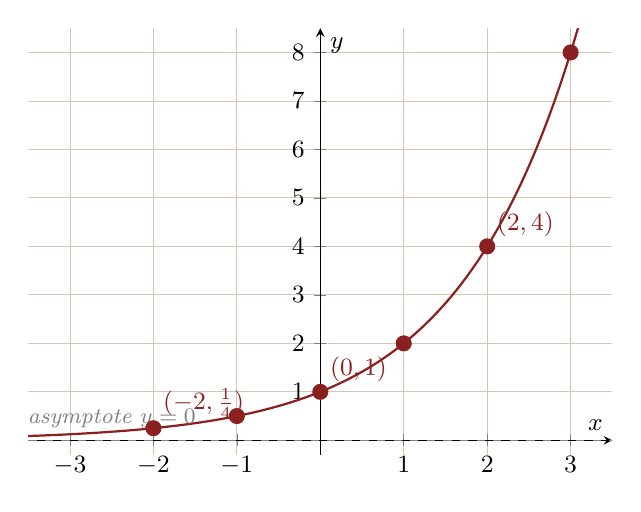
\begin{tikzpicture}
  \begin{axis}[
    width=9cm, height=7cm,
    xlabel={$x$}, ylabel={$y$},
    xmin=-3.5, xmax=3.5,
    ymin=-0.3, ymax=8.5,
    axis lines=center,
    xtick={-3,-2,...,3},
    ytick={1,2,3,4,5,6,7,8},
    grid=both,
    grid style={draw=LightRule, line width=0.3pt},
    tick label style={font=\small},
    label style={font=\small\itshape},
    every axis plot post/.append style={thick},
  ]
    \addplot[domain=-3.5:3.2, samples=120, color=AccentRed, line width=1.8pt]
      {2^x};
    % Key points
    \addplot[only marks, mark=*, mark size=2.5pt, color=AccentRed]
      coordinates {(-2,0.25)(-1,0.5)(0,1)(1,2)(2,4)(3,8)};
    \node[above right, font=\small\itshape, color=AccentRed] at (axis cs:2,4) {$(2,4)$};
    \node[above right, font=\small\itshape, color=AccentRed] at (axis cs:0,1) {$(0,1)$};
    \node[above right, font=\small\itshape, color=AccentRed] at (axis cs:-2,0.25) {$(-2,\tfrac{1}{4})$};
    % Asymptote label
    \draw[dashed, color=gray] (axis cs:-3.5,0) -- (axis cs:3.5,0);
    \node[above, font=\footnotesize\itshape, color=gray] at (axis cs:-2.5,0.05)
      {asymptote $y=0$};
  \end{axis}
\end{tikzpicture}
\end{center}

\subsection*{End Behavior}

\begin{center}
\begin{tabular}{p{0.44\textwidth} p{0.44\textwidth}}
\begin{tcolorbox}[colback=red!5, colframe=red!60!black, arc=4pt,
                  title={\small As $x \to -\infty$}, fonttitle=\bfseries]
  \centering $y \to 0$\\[4pt]
  \small\itshape The curve approaches --- but never touches --- the $x$-axis
  (horizontal asymptote at $y=0$)
\end{tcolorbox}
&
\begin{tcolorbox}[colback=green!5, colframe=green!50!black, arc=4pt,
                  title={\small As $x \to +\infty$}, fonttitle=\bfseries]
  \centering $y \to +\infty$\\[4pt]
  \small\itshape The curve shoots upward without bound (exponential growth)
\end{tcolorbox}
\end{tabular}
\end{center}

\begin{storybox}
\textbf{Linear vs.\ Exponential.}\enspace
Compare $y = 2x+3$ (a straight line: equal changes in $x$ produce \emph{equal}
changes in $y$) with $y = 2^x$ (a curve: equal changes in $x$ produce
\emph{multiplied} changes in $y$). This difference between \emph{additive} and
\emph{multiplicative} growth is one of the most important distinctions in all of
mathematics.
\end{storybox}

\newpage
% ============================================================
%  WORKSHEET
% ============================================================
\section*{Chapter 8 Practice Worksheet}
\addcontentsline{toc}{section}{Chapter 8 Practice Worksheet}

\begin{center}
  {\large\bfseries Exponents, Radicals \& Exponential Functions}\\[6pt]
  \begin{tabular}{lll}
    Name: \shortansline & Date: \shortansline & Score: \shortansline / 20
  \end{tabular}
\end{center}

\vspace{6pt}
\hrule height 1.5pt
\vspace{10pt}

% ── Part A ──────────────────────────────────────────────────
\subsection*{Part A \quad Laws of Exponents \hfill (2 pts each)}
\textit{Simplify each expression. Leave answers with positive exponents only.}

\begin{enumerate}[label=\textbf{\arabic*.}, leftmargin=*, itemsep=18pt]

\item $3^2 \cdot 3^5 = $ \ansline

\item $(5^2)^3 = $ \ansline

\item $7^0 = $ \ansline

\item $4^{-3} = $ \ansline

\item $(2^4)^2 \cdot 2^{-3} = $ \ansline

\end{enumerate}

\vspace{12pt}
% ── Part B ──────────────────────────────────────────────────
\subsection*{Part B \quad Radicals \& Rational Exponents \hfill (2 pts each)}

\begin{enumerate}[label=\textbf{\arabic*.}, leftmargin=*, itemsep=18pt,
                  start=6]

\item Evaluate: \quad $\nthroot{10}{1024} = $ \ansline

\item Write as a radical: \quad $8^{1/3} = $ \ansline

\item Write as a rational exponent: \quad $\nthroot{4}{x^3} = $ \ansline

\item Evaluate: \quad $27^{2/3} = $ \ansline
      \hfill {\small\itshape Hint: find the cube root first}

\item True or False:\quad $\nthroot{n}{a} = a^{1/n}$ \quad \shortansline

\end{enumerate}

\vspace{12pt}
% ── Part C ──────────────────────────────────────────────────
\subsection*{Part C \quad Exponential Function $y = 2^x$ \hfill (short answer)}

\begin{enumerate}[label=\textbf{\arabic*.}, leftmargin=*, itemsep=14pt,
                  start=11]

\item Complete the table of values for $y = 2^x$:

\medskip
\begin{center}
\begin{tabular}{|c|c|c|c|c|c|c|}
  \hline
  $x$       & $-3$ & $-1$ & $0$ & $1$ & $3$ & $4$ \\
  \hline
  $y = 2^x$ & \quad\quad & \quad\quad & \quad\quad & \quad\quad & \quad\quad & \quad\quad \\[12pt]
  \hline
\end{tabular}
\end{center}

\item State the domain and range of $y = 2^x$:

\medskip
Domain: \shortansline \qquad Range: \shortansline

\item Describe the end behavior of $y = 2^x$ in your own words:

\medskip
\ansline

\vspace{6pt}
\ansline

\item Sketch the graph of $y = 2^x$ on the axes below. Label at least three points.

\medskip
\begin{center}
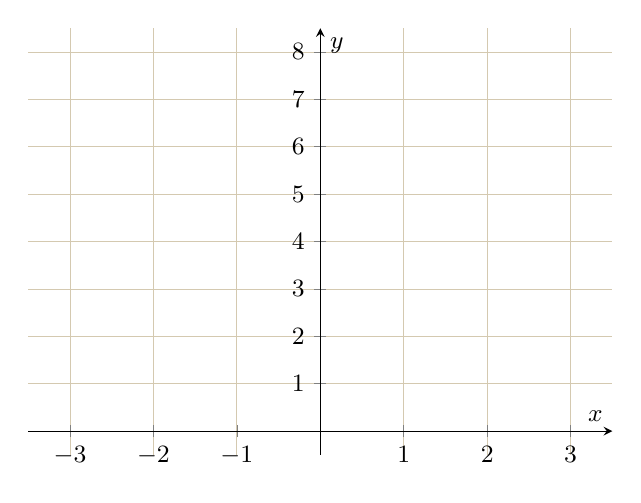
\begin{tikzpicture}
  \begin{axis}[
    width=9cm, height=7cm,
    xlabel={$x$}, ylabel={$y$},
    xmin=-3.5, xmax=3.5, ymin=-0.5, ymax=8.5,
    axis lines=center,
    xtick={-3,-2,...,3}, ytick={0,1,...,8},
    grid=both,
    grid style={draw=LightRule, line width=0.3pt},
    tick label style={font=\small},
    label style={font=\small\itshape},
  ]
  % Empty axes for student to sketch on
  \end{axis}
\end{tikzpicture}
\end{center}

\item \textit{Challenge.}\enspace
If $y = 2^x$ passes through the point $(10,\,1024)$, write this relationship
using \emph{radical notation} and using \emph{rational exponent notation}:

\medskip
Radical: \quad $\nthroot{\phantom{0}}{\ \phantom{000}\ } = $ \shortansline
\qquad
Rational exponent: \quad $(1024)^{\phantom{1/10}} = $ \shortansline

\end{enumerate}

\newpage
% ============================================================
%  ANSWER KEY
% ============================================================
\section*{Answer Key}
\addcontentsline{toc}{section}{Answer Key}

\begin{answerbox}[Part A --- Laws of Exponents]
\begin{enumerate}[label=\textbf{\arabic*.}, noitemsep]
  \item $3^7 = 2187$
  \item $5^6 = 15{,}625$
  \item $1$
  \item $\dfrac{1}{64}$
  \item $2^5 = 32$
\end{enumerate}
\end{answerbox}

\vspace{10pt}

\begin{answerbox}[Part B --- Radicals \& Rational Exponents]
\begin{enumerate}[label=\textbf{\arabic*.}, noitemsep, start=6]
  \item $2$
  \item $\nthroot{3}{8} = 2$
  \item $x^{3/4}$
  \item $\left(\nthroot{3}{27}\right)^2 = 3^2 = 9$
  \item True
\end{enumerate}
\end{answerbox}

\vspace{10pt}

\begin{answerbox}[Part C --- Exponential Function]
\begin{enumerate}[label=\textbf{\arabic*.}, noitemsep, start=11]
  \item $y$ values: $\tfrac{1}{8},\; \tfrac{1}{2},\; 1,\; 2,\; 8,\; 16$
  \item Domain: $(-\infty,+\infty)$;\quad Range: $(0,+\infty)$
  \item As $x \to -\infty$, $y \to 0$ (curve approaches but never touches $x$-axis).
        As $x \to +\infty$, $y \to +\infty$ (exponential growth).
  \item Curve passes through $(-2,\tfrac{1}{4})$, $(0,1)$, $(1,2)$, $(2,4)$;
        rises steeply to the right, flattens toward $y=0$ to the left.
  \item Radical: $\nthroot{10}{1024} = 2$;\quad
        Rational exponent: $1024^{1/10} = 2$
\end{enumerate}
\end{answerbox}

\end{document}
